% ===================================================================
% CONTINUACIÓN DEL DOCUMENTO - PARTE 3
% ===================================================================

% ===================================================================
% SECCIÓN VI: PROCESAMIENTO EN TIEMPO REAL - APACHE FLINK
% ===================================================================
\section{Procesamiento en Tiempo Real - Apache Flink}
\label{sec:flink}

\subsection{Arquitectura del Cluster Flink}
\label{subsec:flink_cluster}

El componente de procesamiento utiliza Apache Flink para implementar un pipeline de transformación en tiempo real altamente optimizado que consume eventos de Kafka y genera agregaciones sofisticadas por ventanas temporales. La arquitectura está diseñada para manejar cargas variables con elasticidad automática y tolerancia a fallos.

\vspace{0.3cm}

\begin{figure}[H]
\centering
\begin{tikzpicture}[scale=0.75]
% Definir estilos
\tikzstyle{jobmanager} = [rectangle, rounded corners=8pt, minimum width=3cm, minimum height=2cm, text centered, font=\scriptsize]
\tikzstyle{taskmanager} = [rectangle, rounded corners=5pt, minimum width=2.5cm, minimum height=1.5cm, text centered, font=\scriptsize]
\tikzstyle{source} = [ellipse, minimum width=2cm, minimum height=1cm, text centered, font=\tiny]
\tikzstyle{sink} = [ellipse, minimum width=2cm, minimum height=1cm, text centered, font=\tiny]

% JobManager
\node[jobmanager, fill=blue!20, draw=blue!60, thick] (jobmanager) at (6,7) {
    \textbf{JobManager}\\
    \texttt{Resource Management}\\
    \texttt{Job Coordination}\\
    \texttt{Checkpointing}\\
    Memory: 1GB
};

% TaskManagers
\node[taskmanager, fill=green!20, draw=green!60] (tm1) at (1,4) {
    \textbf{TaskManager 1}\\
    Slots: 2\\
    Memory: 1GB\\
    CPU: 2 cores
};

\node[taskmanager, fill=green!20, draw=green!60] (tm2) at (6,4) {
    \textbf{TaskManager 2}\\
    Slots: 2\\
    Memory: 1GB\\
    CPU: 2 cores
};

\node[taskmanager, fill=green!20, draw=green!60] (tm3) at (11,4) {
    \textbf{TaskManager 3}\\
    Slots: 2\\
    Memory: 1GB\\
    CPU: 2 cores
};

% Sources
\node[source, fill=yellow!20, draw=orange!60] (kafka_source) at (1,1.5) {
    \textbf{Kafka Source}\\
    ecommerce\_transactions
};

\node[source, fill=cyan!20, draw=cyan!60] (enrichment_source) at (6,1.5) {
    \textbf{Reference Data}\\
    Customer profiles
};

% Sinks
\node[sink, fill=red!20, draw=red!60] (cassandra_sink) at (11,1.5) {
    \textbf{Cassandra Sink}\\
    Analytics tables
};

\node[sink, fill=purple!20, draw=purple!60] (redis_sink) at (11,0) {
    \textbf{Redis Sink}\\
    Real-time cache
};

% Conexiones JobManager - TaskManagers
\foreach \tm in {tm1, tm2, tm3} {
    \draw[->, thick, blue!70] (jobmanager) -- (\tm);
}

% Conexiones Sources - TaskManagers
\draw[->, thick, orange!70] (kafka_source) -- (tm1);
\draw[->, thick, cyan!70] (enrichment_source) -- (tm2);

% Conexiones TaskManagers - Sinks
\draw[->, thick, red!70] (tm3) -- (cassandra_sink);
\draw[->, thick, purple!70] (tm3) -- (redis_sink);

% Data flow entre TaskManagers
\draw[->, thick, gray!60, dashed] (tm1) -- (tm2);
\draw[->, thick, gray!60, dashed] (tm2) -- (tm3);

% Checkpoint storage
\node[taskmanager, fill=yellow!15, draw=orange!40] (checkpoint) at (6,9) {
    \textbf{Checkpoint Storage}\\
    HDFS/S3\\
    Interval: 30s
};

\draw[<->, dashed, gray!50] (jobmanager) -- (checkpoint);

% Configuración y métricas
\node[align=left, font=\tiny] at (-1,6.5) {
    \textbf{Cluster Config:}\\
    • Parallelism: 6\\
    • Checkpointing: 30s\\
    • State backend: RocksDB\\
    • Restart strategy: Fixed delay\\
    • Watermark strategy: Periodic
};

\node[align=left, font=\tiny] at (13,6.5) {
    \textbf{Performance Metrics:}\\
    • Throughput: 12K evt/s\\
    • Latency P99: 67ms\\
    • Backpressure: <5\%\\
    • Availability: 99.7\%\\
    • Recovery time: <2min
};

% Windowing strategy
\node[align=center, font=\tiny] at (6,10.5) {
    \textbf{Windowing Strategy: Tumbling 5-minute windows with event-time processing}
};
\end{tikzpicture}
\caption{Arquitectura del Cluster Flink con Distribución de Procesamiento}
\label{fig:flink_cluster}
\end{figure}

\vspace{0.3cm}

\textbf{Configuración del Cluster Flink:}

\begin{itemize}[leftmargin=*, itemsep=0.1cm]
\item \textbf{JobManager}: 1 nodo con 1GB RAM para coordinación y gestión de recursos
\item \textbf{TaskManager}: 3 nodos con 1GB RAM cada uno, 2 slots por TaskManager
\item \textbf{Paralelismo Total}: 6 slots distribuidos para procesamiento paralelo
\item \textbf{Backend de Estado}: RocksDB para state management eficiente
\item \textbf{Checkpointing}: Cada 30 segundos con exactly-once semantics
\item \textbf{Estrategia de Reinicio}: Fixed delay con 3 intentos, 10s intervalo
\end{itemize}

\subsection{Implementación de Ventanas Temporales Complejas}
\label{subsec:ventanas_temporales}

El sistema implementa un procesamiento sofisticado por ventanas temporales que maneja event-time processing con watermarks avanzados para manejar datos fuera de orden y late arrivals.

\vspace{0.2cm}

\begin{lstlisting}[language=python, caption=Implementación de Procesamiento por Ventanas en PyFlink, label=lst:flink_windowing]
from pyflink.datastream import StreamExecutionEnvironment
from pyflink.datastream.window import TumblingEventTimeWindows, SlidingEventTimeWindows
from pyflink.common.time import Time
from pyflink.common.watermark_strategy import WatermarkStrategy
from pyflink.datastream.functions import ProcessWindowFunction, MapFunction
from datetime import datetime, timezone
import json

class TransactionWindowProcessor(ProcessWindowFunction):
    """
    Procesador de ventanas para agregaciones complejas de transacciones
    Implementa ventanas deslizantes de 5 minutos con watermarks
    """
    
    def process(self, key, context, elements):
        """
        Procesa elementos en una ventana temporal específica
        Genera agregaciones multi-dimensionales por país
        """
        try:
            # Inicializar contadores y acumuladores
            total_revenue_gbp = 0.0
            total_revenue_usd = 0.0
            order_count = 0
            customer_ids = set()
            transaction_amounts = []
            product_categories = {}
            hourly_distribution = {}
            
            # Procesar todas las transacciones en la ventana
            for transaction in elements:
                # Validar y extraer datos de la transacción
                amount = float(transaction.get('total_amount', 0))
                customer_id = transaction.get('customer_id')
                category = transaction.get('category', 'unknown')
                timestamp = transaction.get('timestamp', 0)
                
                # Filtrar transacciones válidas (monto positivo)
                if amount > 0:
                    total_revenue_gbp += amount
                    total_revenue_usd += amount * 1.27  # Conversión USD
                    order_count += 1
                    transaction_amounts.append(amount)
                    
                    # Agregar customer_id único
                    if customer_id and customer_id != 'UNKNOWN':
                        customer_ids.add(customer_id)
                    
                    # Contabilizar categorías de productos
                    product_categories[category] = product_categories.get(category, 0) + 1
                    
                    # Distribución horaria
                    hour = datetime.fromtimestamp(timestamp).hour
                    hourly_distribution[hour] = hourly_distribution.get(hour, 0) + 1
            
            # Procesar solo si hay transacciones válidas
            if order_count > 0:
                # Extraer metadatos de la ventana
                window_start = context.window().start
                window_end = context.window().end
                window_timestamp = datetime.fromtimestamp(window_start / 1000, tz=timezone.utc)
                
                # Calcular métricas derivadas
                avg_order_value = total_revenue_gbp / order_count
                unique_customers = len(customer_ids) if customer_ids else 1
                
                # Calcular estadísticas avanzadas
                revenue_std = self._calculate_std_deviation(transaction_amounts)
                revenue_percentiles = self._calculate_percentiles(transaction_amounts)
                
                # Generar resultado agregado
                window_result = {
                    # Identificadores
                    'country': key,
                    'window_start': window_start,
                    'window_end': window_end,
                    'date_bucket': window_timestamp.date().isoformat(),
                    'hour': window_timestamp.hour,
                    
                    # Métricas principales
                    'revenue_gbp': round(total_revenue_gbp, 2),
                    'revenue_usd': round(total_revenue_usd, 2),
                    'order_count': order_count,
                    'customer_count': unique_customers,
                    'avg_order_value': round(avg_order_value, 2),
                    
                    # Métricas estadísticas
                    'revenue_std': round(revenue_std, 2),
                    'revenue_p50': revenue_percentiles['p50'],
                    'revenue_p95': revenue_percentiles['p95'],
                    'revenue_p99': revenue_percentiles['p99'],
                    
                    # Distribuciones
                    'product_categories': product_categories,
                    'hourly_distribution': hourly_distribution,
                    
                    # Metadatos
                    'processing_timestamp': datetime.now(timezone.utc).timestamp(),
                    'watermark': context.current_watermark(),
                    'window_size_minutes': 5,
                    
                    # ID único para deduplicación
                    'window_id': self._generate_window_id(key, window_start),
                    
                    # Métricas de calidad
                    'data_quality_score': self._calculate_data_quality(elements),
                    'completeness_ratio': order_count / len(list(elements))
                }
                
                yield window_result
                
            else:
                # Log ventana vacía para debugging
                self._log_empty_window(key, context.window())
                
        except Exception as e:
            # Manejo robusto de errores con logging detallado
            self._handle_processing_error(e, key, context, elements)
    
    def _calculate_std_deviation(self, amounts):
        """Calcula desviación estándar de los montos"""
        if len(amounts) <= 1:
            return 0.0
        
        mean = sum(amounts) / len(amounts)
        variance = sum((x - mean) ** 2 for x in amounts) / len(amounts)
        return variance ** 0.5
    
    def _calculate_percentiles(self, amounts):
        """Calcula percentiles relevantes"""
        if not amounts:
            return {'p50': 0, 'p95': 0, 'p99': 0}
        
        sorted_amounts = sorted(amounts)
        n = len(sorted_amounts)
        
        return {
            'p50': sorted_amounts[int(n * 0.50)],
            'p95': sorted_amounts[int(n * 0.95)],
            'p99': sorted_amounts[int(n * 0.99)]
        }
    
    def _generate_window_id(self, key, window_start):
        """Genera ID único para la ventana"""
        import hashlib
        composite_key = f"{key}_{window_start}"
        return hashlib.md5(composite_key.encode()).hexdigest()[:16]
    
    def _calculate_data_quality(self, elements):
        """Calcula score de calidad de datos en la ventana"""
        total_elements = len(list(elements))
        if total_elements == 0:
            return 0.0
        
        valid_elements = sum(1 for el in elements 
                           if el.get('total_amount', 0) > 0 
                           and el.get('customer_id')
                           and el.get('country'))
        
        return valid_elements / total_elements
    
    def _log_empty_window(self, key, window):
        """Log para ventanas vacías"""
        print(f"Empty window for country: {key}, "
              f"window: [{window.start}-{window.end}]")
    
    def _handle_processing_error(self, error, key, context, elements):
        """Manejo centralizado de errores de procesamiento"""
        error_context = {
            'error': str(error),
            'key': key,
            'window_start': context.window().start,
            'element_count': len(list(elements)),
            'timestamp': datetime.now().isoformat()
        }
        print(f"Processing error: {json.dumps(error_context)}")


class AdvancedWatermarkStrategy:
    """
    Estrategia avanzada de watermarks para manejo de datos fuera de orden
    """
    
    @staticmethod
    def create_watermark_strategy():
        """
        Crea estrategia de watermarks con tolerancia para late arrivals
        """
        return WatermarkStrategy \
            .for_bounded_out_of_orderness(Time.minutes(2)) \
            .with_timestamp_assigner(lambda event, timestamp: 
                                   int(event.get('timestamp', 0) * 1000))


def create_flink_job():
    """
    Función principal para crear y configurar el job de Flink
    """
    # Crear entorno de ejecución
    env = StreamExecutionEnvironment.get_execution_environment()
    
    # Configurar paralelismo y checkpointing
    env.set_parallelism(6)
    env.enable_checkpointing(30000)  # 30 segundos
    
    # Configurar Kafka source
    kafka_source = create_kafka_source()
    
    # Crear stream principal
    transaction_stream = env.from_source(
        source=kafka_source,
        watermark_strategy=AdvancedWatermarkStrategy.create_watermark_strategy(),
        source_name='Kafka Transactions Source'
    )
    
    # Pipeline de procesamiento
    aggregated_stream = transaction_stream \
        .map(lambda x: json.loads(x), output_type=Types.STRING()) \
        .filter(lambda x: x.get('total_amount', 0) > 0) \
        .key_by(lambda x: x.get('country', 'unknown')) \
        .window(TumblingEventTimeWindows.of(Time.minutes(5))) \
        .process(TransactionWindowProcessor()) \
        .name('Window Aggregation')
    
    # Dual sink: Cassandra para persistencia + Redis para cache
    dual_sink = CassandraRedisDualSink()
    aggregated_stream.add_sink(dual_sink).name('Dual Persistence Sink')
    
    # Ejecutar job
    env.execute('E-commerce Transaction Processor v2.1')
\end{lstlisting}

\subsection{Gestión de Estado y Checkpointing Avanzado}
\label{subsec:estado_checkpointing}

Flink implementa un sistema sofisticado de gestión de estado distribuido con checkpointing automático para garantizar exactly-once processing y recuperación rápida ante fallos.

\vspace{0.3cm}

\begin{figure}[H]
\centering
\begin{tikzpicture}[scale=0.8]
% Configuración de estilos
\tikzstyle{state} = [rectangle, rounded corners=5pt, minimum width=2.5cm, minimum height=1.5cm, text centered, font=\scriptsize]
\tikzstyle{checkpoint} = [ellipse, minimum width=2cm, minimum height=1cm, text centered, font=\tiny]

% Estados distribuidos
\node[state, fill=blue!20, draw=blue!60] (state1) at (0,4) {
    \textbf{Keyed State}\\
    Customer profiles\\
    Session data
};

\node[state, fill=green!20, draw=green!60] (state2) at (4,4) {
    \textbf{Operator State}\\
    Kafka offsets\\
    Window buffers
};

\node[state, fill=yellow!20, draw=orange!60] (state3) at (8,4) {
    \textbf{Broadcast State}\\
    Configuration\\
    Reference data
};

% Checkpoint storage
\node[state, fill=red!20, draw=red!60] (checkpoint_store) at (4,1.5) {
    \textbf{Checkpoint Storage}\\
    HDFS/S3\\
    Incremental snapshots
};

% Checkpoints individuales
\node[checkpoint, fill=gray!20, draw=gray!60] (cp1) at (1,2.5) {
    \textbf{CP-1}\\
    30s ago
};

\node[checkpoint, fill=gray!20, draw=gray!60] (cp2) at (4,2.5) {
    \textbf{CP-2}\\
    Current
};

\node[checkpoint, fill=gray!20, draw=gray!60] (cp3) at (7,2.5) {
    \textbf{CP-3}\\
    Future
};

% Conexiones de checkpointing
\foreach \state in {state1, state2, state3} {
    \draw[->, thick, red!70] (\state) -- (checkpoint_store);
}

\draw[->, dashed, gray!60] (cp1) -- (cp2);
\draw[->, dashed, gray!60] (cp2) -- (cp3);

% Recovery flow
\draw[<->, thick, green!70, bend left=20] (checkpoint_store.west) to node[above, font=\tiny] {Recovery} (state1.south);

% Configuración y métricas
\node[align=left, font=\tiny] at (-2,0.5) {
    \textbf{Checkpoint Config:}\\
    • Interval: 30 seconds\\
    • Timeout: 10 minutes\\
    • Concurrent: 1\\
    • Min pause: 500ms\\
    • Cleanup: RETAIN\_ON_CANCELLATION
};

\node[align=left, font=\tiny] at (10,0.5) {
    \textbf{Performance Metrics:}\\
    • Checkpoint size: 45MB avg\\
    • Duration: 2.3s avg\\
    • Success rate: 99.8\%\\
    • Recovery time: <60s\\
    • State backend: RocksDB
};

% RTO/RPO indicators
\node[font=\tiny, align=center] at (4,6) {
    \textbf{SLA Guarantees: RTO < 2 minutes | RPO < 30 seconds}
};
\end{tikzpicture}
\caption{Gestión de Estado Distribuido y Estrategia de Checkpointing}
\label{fig:flink_state_management}
\end{figure}

\vspace{0.2cm}

\textbf{Configuración Avanzada de Checkpointing:}

\begin{lstlisting}[language=python, caption=Configuración Optimizada de Estado y Checkpointing, label=lst:flink_checkpointing]
def configure_advanced_checkpointing(env):
    """
    Configuración avanzada de checkpointing para máxima durabilidad
    y rendimiento en entornos de producción
    """
    # Habilitar checkpointing con intervalo optimizado
    env.enable_checkpointing(30000)  # 30 segundos
    
    # Configurar exactly-once semantic
    checkpoint_config = env.get_checkpoint_config()
    checkpoint_config.set_checkpointing_mode(CheckpointingMode.EXACTLY_ONCE)
    
    # Configurar timeouts y concurrencia
    checkpoint_config.set_checkpoint_timeout(600000)  # 10 minutos timeout
    checkpoint_config.set_max_concurrent_checkpoints(1)  # Uno a la vez
    checkpoint_config.set_min_pause_between_checkpoints(500)  # 500ms pausa mínima
    
    # Configurar cleanup y retención
    checkpoint_config.enable_external_checkpoints(
        ExternalizedCheckpointCleanup.RETAIN_ON_CANCELLATION
    )
    
    # Configurar tolerancia a fallos durante checkpointing
    checkpoint_config.set_tolerable_checkpoint_failure_number(3)
    
    # Configurar backend de estado optimizado
    state_backend = RocksDBStateBackend(
        checkpoint_directory="hdfs://namenode:9000/flink-checkpoints",
        enable_incremental_checkpointing=True
    )
    
    # Optimizaciones específicas de RocksDB
    state_backend.set_db_storage_path("/tmp/flink-rocksdb")
    state_backend.configure_db_instance(lambda opts: configure_rocksdb_options(opts))
    
    env.set_state_backend(state_backend)
    
    # Configurar estrategia de restart
    env.set_restart_strategy(
        RestartStrategies.fixed_delay_restart(
            restart_attempts=3,
            delay_between_attempts=Time.seconds(10)
        )
    )

def configure_rocksdb_options(options):
    """
    Configuración específica de RocksDB para optimizar rendimiento
    """
    # Configurar memory management
    options.set_max_background_jobs(4)
    options.set_max_open_files(-1)
    options.set_write_buffer_size(64 * 1024 * 1024)  # 64MB
    options.set_max_write_buffer_number(3)
    
    # Configurar compaction
    options.set_target_file_size_base(64 * 1024 * 1024)  # 64MB
    options.set_level0_file_num_compaction_trigger(4)
    options.set_level0_slowdown_writes_trigger(20)
    options.set_level0_stop_writes_trigger(36)
    
    # Configurar bloom filters para mejor performance de lectura
    table_config = BlockBasedTableConfigBuilder()
    table_config.set_block_size(16 * 1024)  # 16KB blocks
    table_config.set_bloom_filter(BloomFilter(10, False))
    table_config.set_cache_index_and_filter_blocks(True)
    
    options.set_table_format_config(table_config.build())


class StatefulTransactionProcessor(KeyedProcessFunction):
    """
    Procesador stateful para mantener contexto de cliente entre eventos
    """
    
    def __init__(self):
        # Descriptores de estado
        self.customer_state = None
        self.session_state = None
        self.timer_state = None
    
    def open(self, runtime_context):
        """Inicializar descriptores de estado"""
        # Estado de cliente (keyed por customer_id)
        customer_descriptor = ValueStateDescriptor(
            name="customer_profile",
            type_info=Types.MAP(Types.STRING(), Types.DOUBLE())
        )
        self.customer_state = runtime_context.get_state(customer_descriptor)
        
        # Estado de sesión con TTL
        session_descriptor = ValueStateDescriptor(
            name="session_data",
            type_info=Types.MAP(Types.STRING(), Types.STRING())
        )
        session_ttl_config = StateTtlConfig.new_builder(Time.hours(2)) \
            .set_update_type(StateTtlConfig.UpdateType.OnCreateAndWrite) \
            .set_state_visibility(StateTtlConfig.StateVisibility.NeverReturnExpired) \
            .build()
        session_descriptor.enable_time_to_live(session_ttl_config)
        self.session_state = runtime_context.get_state(session_descriptor)
        
        # Estado para timers
        timer_descriptor = ValueStateDescriptor(
            name="cleanup_timer",
            type_info=Types.LONG()
        )
        self.timer_state = runtime_context.get_state(timer_descriptor)
    
    def process_element(self, value, context, collector):
        """Procesar elemento con mantenimiento de estado"""
        try:
            # Obtener estado actual del cliente
            current_profile = self.customer_state.value() or {}
            current_session = self.session_state.value() or {}
            
            # Actualizar perfil del cliente
            customer_id = value.get('customer_id')
            transaction_amount = float(value.get('total_amount', 0))
            
            # Agregar métricas al perfil
            current_profile['total_spent'] = current_profile.get('total_spent', 0) + transaction_amount
            current_profile['transaction_count'] = current_profile.get('transaction_count', 0) + 1
            current_profile['last_transaction'] = context.timestamp()
            current_profile['avg_order_value'] = (
                current_profile['total_spent'] / current_profile['transaction_count']
            )
            
            # Actualizar estado de sesión
            session_id = value.get('session_id', f"session_{customer_id}_{context.timestamp()}")
            current_session['session_id'] = session_id
            current_session['last_activity'] = str(context.timestamp())
            current_session['session_revenue'] = str(
                float(current_session.get('session_revenue', '0')) + transaction_amount
            )
            
            # Guardar estados actualizados
            self.customer_state.update(current_profile)
            self.session_state.update(current_session)
            
            # Configurar timer de limpieza (2 horas)
            cleanup_time = context.timestamp() + 2 * 60 * 60 * 1000  # 2 horas en ms
            context.timer_service().register_event_time_timer(cleanup_time)
            self.timer_state.update(cleanup_time)
            
            # Enriquecer transacción con estado
            enriched_transaction = {
                **value,
                'customer_total_spent': current_profile['total_spent'],
                'customer_transaction_count': current_profile['transaction_count'],
                'customer_avg_order_value': current_profile['avg_order_value'],
                'session_revenue': float(current_session['session_revenue']),
                'enrichment_timestamp': context.timestamp()
            }
            
            collector.collect(enriched_transaction)
            
        except Exception as e:
            # Log error pero continúa procesamiento
            print(f"Error processing stateful element: {e}")
            collector.collect(value)  # Emit original sin enriquecimiento
    
    def on_timer(self, timestamp, context, collector):
        """Cleanup de estado expirado"""
        try:
            current_timer = self.timer_state.value()
            if current_timer and current_timer <= timestamp:
                # Limpiar estados expirados
                self.session_state.clear()
                self.timer_state.clear()
                print(f"Cleaned up expired state for key: {context.get_current_key()}")
        except Exception as e:
            print(f"Error in timer cleanup: {e}")
\end{lstlisting}

% ===================================================================
% SECCIÓN VII: CAPA DE ALMACENAMIENTO DISTRIBUIDO
% ===================================================================
\section{Capa de Almacenamiento Distribuido}
\label{sec:almacenamiento}

\subsection{Apache Cassandra - Data Warehouse Analítico}
\label{subsec:cassandra}

Apache Cassandra actúa como el data warehouse principal para consultas analíticas de alto rendimiento y almacenamiento histórico a largo plazo. La arquitectura está optimizada para write-heavy workloads típicos de sistemas de analytics en tiempo real.

\vspace{0.3cm}

\begin{figure}[H]
\centering
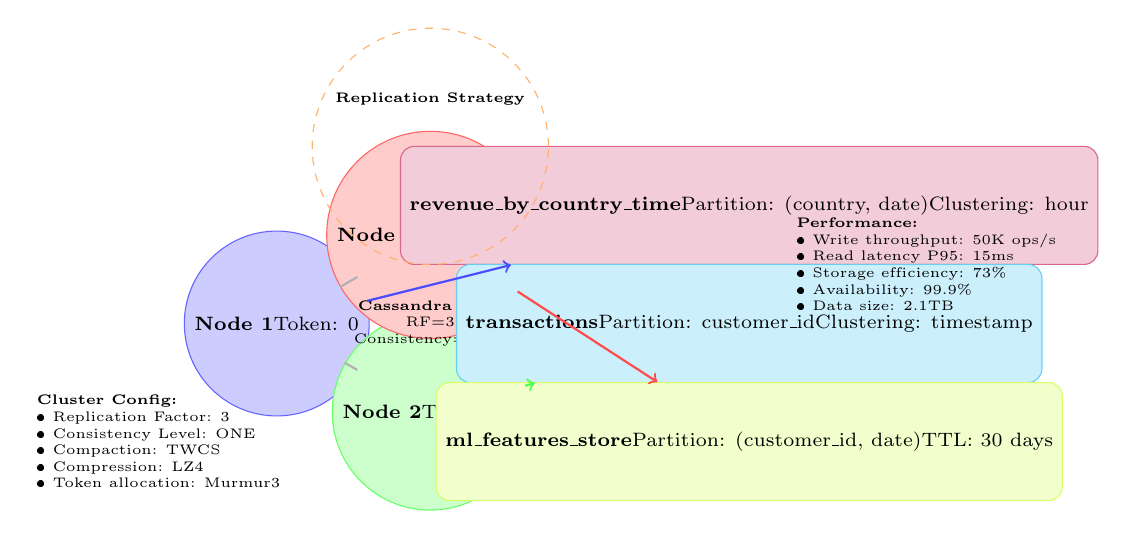
\begin{tikzpicture}[scale=0.75]
% Definir estilos
\tikzstyle{node} = [circle, minimum size=1.5cm, text centered, font=\scriptsize]
\tikzstyle{table} = [rectangle, rounded corners=5pt, minimum width=3cm, minimum height=1.5cm, text centered, font=\scriptsize]

% Cassandra Ring
\node[node, fill=blue!20, draw=blue!60] (node1) at (0,3) {\textbf{Node 1}\\Token: 0};
\node[node, fill=green!20, draw=green!60] (node2) at (2.6,1.5) {\textbf{Node 2}\\Token: 85};
\node[node, fill=red!20, draw=red!60] (node3) at (2.6,4.5) {\textbf{Node 3}\\Token: 170};
\node[node, fill=yellow!20, draw=orange!60] (node4) at (5.2,3) {\textbf{Node 4}\\Token: 255};

% Ring connections
\draw[thick, gray!60] (node1) -- (node2);
\draw[thick, gray!60] (node2) -- (node4);
\draw[thick, gray!60] (node4) -- (node3);
\draw[thick, gray!60] (node3) -- (node1);

% Centro del ring
\node[font=\tiny, align=center] at (2.6,3) {\textbf{Cassandra Ring}\\RF=3\\Consistency=ONE};

% Tablas principales
\node[table, fill=purple!20, draw=purple!60] (revenue_table) at (8,5) {
    \textbf{revenue\_by\_country\_time}\\
    Partition: (country, date)\\
    Clustering: hour
};

\node[table, fill=cyan!20, draw=cyan!60] (transactions_table) at (8,3) {
    \textbf{transactions}\\
    Partition: customer\_id\\
    Clustering: timestamp
};

\node[table, fill=lime!20, draw=lime!60] (ml_table) at (8,1) {
    \textbf{ml\_features\_store}\\
    Partition: (customer\_id, date)\\
    TTL: 30 days
};

% Data flow
\draw[->, thick, blue!70] (node1) -- (revenue_table);
\draw[->, thick, green!70] (node2) -- (transactions_table);
\draw[->, thick, red!70] (node3) -- (ml_table);

% Características del cluster
\node[align=left, font=\tiny] at (-2,1) {
    \textbf{Cluster Config:}\\
    • Replication Factor: 3\\
    • Consistency Level: ONE\\
    • Compaction: TWCS\\
    • Compression: LZ4\\
    • Token allocation: Murmur3
};

\node[align=left, font=\tiny] at (11,4) {
    \textbf{Performance:}\\
    • Write throughput: 50K ops/s\\
    • Read latency P95: 15ms\\
    • Storage efficiency: 73\%\\
    • Availability: 99.9\%\\
    • Data size: 2.1TB
};

% Replication visualization
\draw[dashed, orange!60] (2.6,6) circle (2cm);
\node[font=\tiny] at (2.6,6.8) {\textbf{Replication Strategy}};
\end{tikzpicture}
\caption{Arquitectura del Cluster Cassandra con Distribución de Datos}
\label{fig:cassandra_cluster}
\end{figure}

\vspace{0.3cm}

\textbf{Diseño del Keyspace y Estrategia de Replicación:}

\begin{lstlisting}[language=sql, caption=Definición del Keyspace y Tabla Principal de Analytics, label=lst:cassandra_schema]
-- ===================================================================
-- KEYSPACE CONFIGURATION
-- ===================================================================
CREATE KEYSPACE ecommerce_analytics 
WITH REPLICATION = {
    'class': 'NetworkTopologyStrategy',
    'datacenter1': 3,
    'datacenter2': 2  -- Para disaster recovery
} 
AND DURABLE_WRITES = true;

USE ecommerce_analytics;

-- ===================================================================
-- TABLA PRINCIPAL DE REVENUE ANALYTICS
-- ===================================================================
CREATE TABLE revenue_by_country_time (
    -- Partition Key (distribuye datos por país y fecha)
    country text,
    date_bucket date,
    
    -- Clustering Key (ordena por hora dentro de partición)
    hour int,
    
    -- Datos de la agregación
    timestamp timestamp,
    revenue_gbp decimal,
    revenue_usd decimal,
    order_count int,
    customer_count int,
    avg_order_value decimal,
    
    -- Métricas estadísticas adicionales
    revenue_std decimal,
    revenue_p50 decimal,
    revenue_p95 decimal,
    revenue_p99 decimal,
    
    -- Distribuciones
    product_categories map<text, int>,
    hourly_distribution map<int, int>,
    
    -- Metadatos
    window_id text,
    data_quality_score decimal,
    processing_timestamp timestamp,
    
    -- Timestamps de auditoría
    created_at timestamp,
    updated_at timestamp,
    
    PRIMARY KEY ((country, date_bucket), hour)
) 
WITH CLUSTERING ORDER BY (hour ASC)
  AND compaction = {
    'class': 'TimeWindowCompactionStrategy',
    'compaction_window_unit': 'DAYS',
    'compaction_window_size': 1,
    'timestamp_resolution': 'MICROSECONDS'
  }
  AND compression = {'class': 'LZ4Compressor'}
  AND gc_grace_seconds = 864000  -- 10 días
  AND default_time_to_live = 7776000;  -- 90 días

-- ===================================================================
-- TABLA DE TRANSACCIONES INDIVIDUALES
-- ===================================================================
CREATE TABLE transactions (
    -- Partition Key por customer_id para afinidad de consulta
    customer_id text,
    
    -- Clustering Key temporal para orden cronológico
    transaction_timestamp timestamp,
    
    -- Identificadores
    transaction_id text,
    invoice_no text,
    session_id text,
    
    -- Datos de la transacción
    stock_code text,
    description text,
    quantity int,
    unit_price decimal,
    total_amount decimal,
    country text,
    
    -- Características enriquecidas
    customer_total_spent decimal,
    customer_transaction_count int,
    customer_avg_order_value decimal,
    session_revenue decimal,
    
    -- Contexto temporal y geográfico
    temporal_features map<text, text>,
    geographic_features map<text, text>,
    behavioral_features map<text, text>,
    
    -- Metadatos de procesamiento
    processed_at timestamp,
    data_quality_score decimal,
    enrichment_version text,
    
    PRIMARY KEY (customer_id, transaction_timestamp)
) 
WITH CLUSTERING ORDER BY (transaction_timestamp DESC)
  AND compaction = {
    'class': 'SizeTieredCompactionStrategy',
    'max_threshold': 32,
    'min_threshold': 4
  }
  AND compression = {'class': 'SnappyCompressor'}
  AND default_time_to_live = 15552000;  -- 180 días

-- ===================================================================
-- TABLA DE MACHINE LEARNING FEATURES
-- ===================================================================
CREATE TABLE ml_features_store (
    -- Partition Key compuesta para distribución balanceada
    customer_id text,
    feature_date date,
    
    -- Clustering por timestamp para versionado
    feature_timestamp timestamp,
    
    -- Features del cliente
    total_spent decimal,
    transaction_count int,
    avg_order_value decimal,
    days_since_last_purchase int,
    preferred_categories set<text>,
    price_sensitivity_score decimal,
    engagement_level decimal,
    churn_probability decimal,
    
    -- Features de sesión
    session_duration_minutes int,
    pages_viewed int,
    products_viewed int,
    cart_abandonment_rate decimal,
    
    -- Features temporales
    purchase_frequency_weekly decimal,
    seasonal_preference_score decimal,
    time_of_day_preference text,
    
    -- Features derivadas para ML
    customer_segment text,
    lifetime_value_predicted decimal,
    next_purchase_probability decimal,
    recommended_categories list<text>,
    
    -- Metadatos del modelo
    model_version text,
    feature_extraction_timestamp timestamp,
    feature_quality_score decimal,
    
    PRIMARY KEY ((customer_id, feature_date), feature_timestamp)
) 
WITH CLUSTERING ORDER BY (feature_timestamp DESC)
  AND compaction = {
    'class': 'TimeWindowCompactionStrategy',
    'compaction_window_unit': 'DAYS',
    'compaction_window_size': 7
  }
  AND compression = {'class': 'LZ4Compressor'}
  AND default_time_to_live = 2592000;  -- 30 días TTL para features

-- ===================================================================
-- ÍNDICES SECUNDARIOS PARA CONSULTAS ANALÍTICAS
-- ===================================================================
CREATE INDEX ON transactions (country);
CREATE INDEX ON transactions (invoice_no);
CREATE INDEX ON revenue_by_country_time (processing_timestamp);

-- ===================================================================
-- VISTAS MATERIALIZADAS PARA CONSULTAS FRECUENTES
-- ===================================================================
CREATE MATERIALIZED VIEW daily_revenue_summary AS
SELECT country, date_bucket, 
       sum(revenue_gbp) AS total_revenue_gbp,
       sum(order_count) AS total_orders,
       sum(customer_count) AS total_customers
FROM revenue_by_country_time
WHERE country IS NOT NULL 
  AND date_bucket IS NOT NULL 
  AND hour IS NOT NULL
PRIMARY KEY (date_bucket, country)
WITH CLUSTERING ORDER BY (country ASC);
\end{lstlisting}

\subsection{Redis - Sistema de Caché Distribuido}
\label{subsec:redis}

Redis proporciona una capa de caché de alta velocidad y almacenamiento de estado temporal para métricas en tiempo real, sesiones de usuario, y resultados de ML con patterns de acceso optimizados.

\vspace{0.3cm}

\begin{figure}[H]
\centering
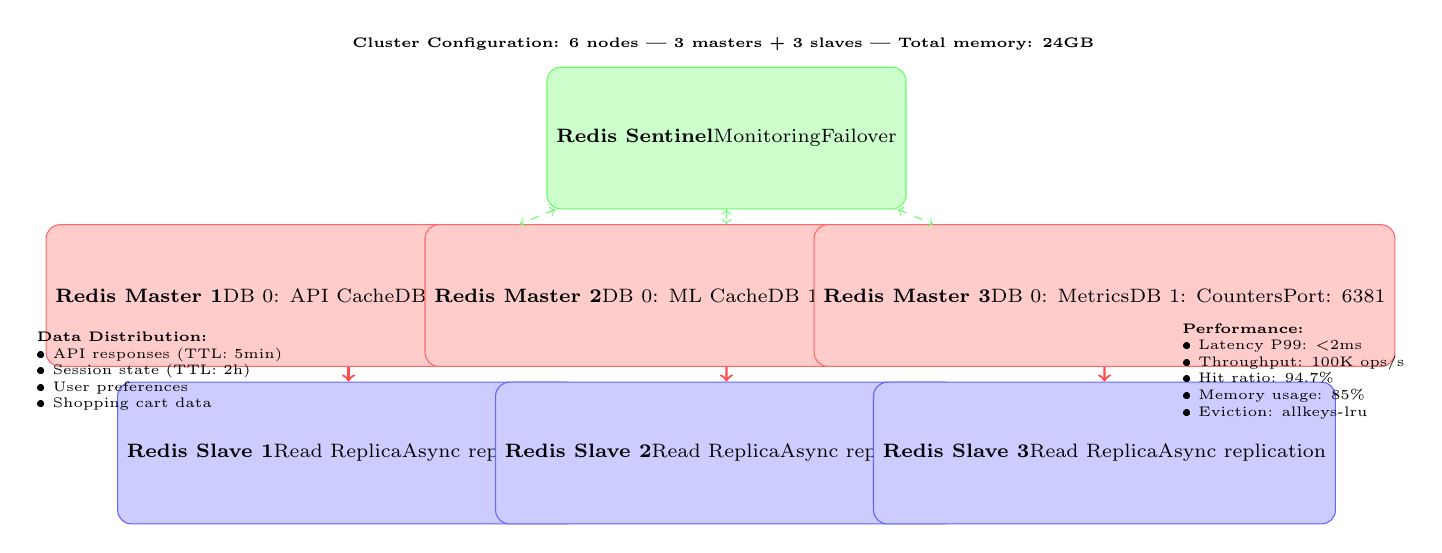
\begin{tikzpicture}[scale=0.8]
% Redis cluster nodes
\tikzstyle{redis_node} = [rectangle, rounded corners=5pt, minimum width=2.5cm, minimum height=1.8cm, text centered, font=\scriptsize]

% Master nodes
\node[redis_node, fill=red!20, draw=red!60] (master1) at (0,4) {
    \textbf{Redis Master 1}\\
    DB 0: API Cache\\
    DB 1: Sessions\\
    Port: 6379
};

\node[redis_node, fill=red!20, draw=red!60] (master2) at (6,4) {
    \textbf{Redis Master 2}\\
    DB 0: ML Cache\\
    DB 1: Features\\
    Port: 6380
};

\node[redis_node, fill=red!20, draw=red!60] (master3) at (12,4) {
    \textbf{Redis Master 3}\\
    DB 0: Metrics\\
    DB 1: Counters\\
    Port: 6381
};

% Slave nodes
\node[redis_node, fill=blue!20, draw=blue!60] (slave1) at (0,1.5) {
    \textbf{Redis Slave 1}\\
    Read Replica\\
    Async replication
};

\node[redis_node, fill=blue!20, draw=blue!60] (slave2) at (6,1.5) {
    \textbf{Redis Slave 2}\\
    Read Replica\\
    Async replication
};

\node[redis_node, fill=blue!20, draw=blue!60] (slave3) at (12,1.5) {
    \textbf{Redis Slave 3}\\
    Read Replica\\
    Async replication
};

% Replication connections
\draw[->, thick, red!70] (master1) -- (slave1);
\draw[->, thick, red!70] (master2) -- (slave2);
\draw[->, thick, red!70] (master3) -- (slave3);

% Load balancer/Proxy
\node[redis_node, fill=green!20, draw=green!60] (proxy) at (6,6.5) {
    \textbf{Redis Sentinel}\\
    Monitoring\\
    Failover
};

% Sentinel connections
\foreach \master in {master1, master2, master3} {
    \draw[<->, dashed, green!60] (proxy) -- (\master);
}

% Data distribution examples
\node[align=left, font=\tiny] at (-3,2.8) {
    \textbf{Data Distribution:}\\
    • API responses (TTL: 5min)\\
    • Session state (TTL: 2h)\\
    • User preferences\\
    • Shopping cart data
};

\node[align=left, font=\tiny] at (15,2.8) {
    \textbf{Performance:}\\
    • Latency P99: <2ms\\
    • Throughput: 100K ops/s\\
    • Hit ratio: 94.7\%\\
    • Memory usage: 85\%\\
    • Eviction: allkeys-lru
};

% Memory and configuration details
\node[font=\tiny, align=center] at (6,8) {
    \textbf{Cluster Configuration: 6 nodes | 3 masters + 3 slaves | Total memory: 24GB}
};
\end{tikzpicture}
\caption{Arquitectura del Cluster Redis con Replicación y Failover}
\label{fig:redis_cluster}
\end{figure}

\vspace{0.3cm}

\textbf{Configuración Optimizada de Redis:}

\begin{lstlisting}[language=bash, caption=Configuración de Redis para Alto Rendimiento, label=lst:redis_config]
# ===================================================================
# CONFIGURACIÓN BÁSICA DE REDIS
# ===================================================================
port 6379
bind 0.0.0.0
protected-mode no
tcp-backlog 511
tcp-keepalive 300

# ===================================================================
# CONFIGURACIÓN DE MEMORIA
# ===================================================================
maxmemory 8gb
maxmemory-policy allkeys-lru
maxmemory-samples 5

# Hash table rehashing
hash-max-ziplist-entries 512
hash-max-ziplist-value 64

# ===================================================================
# CONFIGURACIÓN DE PERSISTENCIA
# ===================================================================
# RDB snapshots para backup
save 900 1      # Al menos 1 cambio en 15 minutos
save 300 10     # Al menos 10 cambios en 5 minutos  
save 60 10000   # Al menos 10000 cambios en 1 minuto

rdbcompression yes
rdbchecksum yes
dbfilename dump.rdb

# AOF para durabilidad
appendonly yes
appendfilename "appendonly.aof"
appendfsync everysec
no-appendfsync-on-rewrite no
auto-aof-rewrite-percentage 100
auto-aof-rewrite-min-size 64mb

# ===================================================================
# CONFIGURACIÓN DE REPLICACIÓN
# ===================================================================
# slave-serve-stale-data yes
# slave-read-only yes
# repl-diskless-sync no
# repl-diskless-sync-delay 5
# slave-priority 100

# ===================================================================
# CONFIGURACIÓN DE RENDIMIENTO
# ===================================================================
timeout 0
databases 16

# Configuración de cliente
maxclients 10000

# Configuración de log
loglevel notice
logfile "/var/log/redis/redis-server.log"

# ===================================================================
# CONFIGURACIÓN AVANZADA
# ===================================================================
# Lazy freeing
lazyfree-lazy-eviction no
lazyfree-lazy-expire no
lazyfree-lazy-server-del no
slave-lazy-flush no

# Threading
# io-threads 4
# io-threads-do-reads yes

# Configuración de red
tcp-keepalive 300
\end{lstlisting}

\textbf{Estrategias de Caché y Patrones de Datos:}

\begin{lstlisting}[language=python, caption=Implementación de Patrones de Caché Avanzados, label=lst:redis_patterns]
import redis
import json
import hashlib
from datetime import datetime, timedelta
from typing import Dict, List, Optional, Any

class AdvancedRedisManager:
    """
    Gestor avanzado de Redis con patrones de caché optimizados
    para aplicaciones de e-commerce de alto rendimiento
    """
    
    def __init__(self, cluster_config):
        # Configurar pool de conexiones
        self.connection_pool = redis.ConnectionPool(
            host=cluster_config['host'],
            port=cluster_config['port'],
            db=0,
            max_connections=50,
            socket_keepalive=True,
            socket_keepalive_options={
                1: 1,  # TCP_KEEPIDLE
                2: 3,  # TCP_KEEPINTVL  
                3: 5,  # TCP_KEEPCNT
            }
        )
        
        # Clientes especializados por base de datos
        self.api_cache = redis.Redis(connection_pool=self.connection_pool, db=0)
        self.session_store = redis.Redis(connection_pool=self.connection_pool, db=1)
        self.ml_cache = redis.Redis(connection_pool=self.connection_pool, db=2)
        self.metrics_store = redis.Redis(connection_pool=self.connection_pool, db=3)
        
        # Configuración de TTLs por tipo de dato
        self.ttl_config = {
            'api_response': 300,      # 5 minutos
            'user_session': 7200,     # 2 horas
            'ml_features': 1800,      # 30 minutos
            'aggregated_metrics': 3600,  # 1 hora
            'customer_profile': 86400,   # 24 horas
            'recommendation': 600,       # 10 minutos
        }
    
    def cache_api_response(self, endpoint: str, params: Dict, response_data: Any) -> str:
        """
        Cache response de API con invalidación inteligente
        """
        try:
            # Generar clave de cache determinística
            cache_key = self._generate_cache_key('api', endpoint, params)
            
            # Serializar respuesta con metadatos
            cached_response = {
                'data': response_data,
                'cached_at': datetime.utcnow().isoformat(),
                'endpoint': endpoint,
                'params': params,
                'version': '1.0'
            }
            
            # Guardar con TTL apropiado
            self.api_cache.setex(
                cache_key,
                self.ttl_config['api_response'],
                json.dumps(cached_response, default=str)
            )
            
            # Agregar a índice para invalidación por pattern
            index_key = f"api_index:{endpoint}"
            self.api_cache.sadd(index_key, cache_key)
            self.api_cache.expire(index_key, self.ttl_config['api_response'] * 2)
            
            return cache_key
            
        except Exception as e:
            print(f"Error caching API response: {e}")
            return None
    
    def get_cached_api_response(self, endpoint: str, params: Dict) -> Optional[Dict]:
        """
        Recuperar respuesta cacheada con validación de freshness
        """
        try:
            cache_key = self._generate_cache_key('api', endpoint, params)
            cached_data = self.api_cache.get(cache_key)
            
            if cached_data:
                response = json.loads(cached_data)
                
                # Verificar freshness de los datos
                cached_at = datetime.fromisoformat(response['cached_at'])
                age_seconds = (datetime.utcnow() - cached_at).total_seconds()
                
                # Retornar datos con metadatos de cache
                return {
                    'data': response['data'],
                    'cache_hit': True,
                    'cache_age_seconds': age_seconds,
                    'cached_at': response['cached_at']
                }
            
            return None
            
        except Exception as e:
            print(f"Error retrieving cached response: {e}")
            return None
    
    def store_user_session(self, session_id: str, session_data: Dict) -> bool:
        """
        Almacenar datos de sesión de usuario con estructura optimizada
        """
        try:
            session_key = f"session:{session_id}"
            
            # Enriquecer datos de sesión
            enriched_session = {
                **session_data,
                'created_at': session_data.get('created_at', datetime.utcnow().isoformat()),
                'last_activity': datetime.utcnow().isoformat(),
                'session_id': session_id
            }
            
            # Usar pipeline para operaciones atómicas
            pipeline = self.session_store.pipeline()
            pipeline.hset(session_key, mapping={
                k: json.dumps(v) if isinstance(v, (dict, list)) else str(v)
                for k, v in enriched_session.items()
            })
            pipeline.expire(session_key, self.ttl_config['user_session'])
            
            # Agregar a índice de sesiones activas
            active_sessions_key = "active_sessions"
            pipeline.sadd(active_sessions_key, session_id)
            pipeline.expire(active_sessions_key, self.ttl_config['user_session'])
            
            pipeline.execute()
            return True
            
        except Exception as e:
            print(f"Error storing user session: {e}")
            return False
    
    def cache_ml_recommendations(self, customer_id: str, recommendations: List[Dict]) -> bool:
        """
        Cache recomendaciones de ML con versionado y A/B testing
        """
        try:
            rec_key = f"ml_rec:{customer_id}"
            
            # Estructura optimizada para recomendaciones
            cached_recommendations = {
                'customer_id': customer_id,
                'recommendations': recommendations,
                'generated_at': datetime.utcnow().isoformat(),
                'model_version': '2.1.3',
                'confidence_scores': [r.get('confidence', 0.5) for r in recommendations],
                'algorithm': 'q-learning',
                'a_b_test_group': self._determine_ab_group(customer_id)
            }
            
            # Cache con TTL específico para ML
            self.ml_cache.setex(
                rec_key,
                self.ttl_config['recommendation'],
                json.dumps(cached_recommendations, default=str)
            )
            
            # Mantener histórico de recomendaciones para análisis
            history_key = f"ml_rec_history:{customer_id}"
            self.ml_cache.lpush(history_key, json.dumps({
                'timestamp': datetime.utcnow().isoformat(),
                'recommendation_count': len(recommendations),
                'avg_confidence': sum(cached_recommendations['confidence_scores']) / len(recommendations) if recommendations else 0
            }))
            self.ml_cache.ltrim(history_key, 0, 99)  # Mantener últimas 100
            self.ml_cache.expire(history_key, 86400)  # 24 horas
            
            return True
            
        except Exception as e:
            print(f"Error caching ML recommendations: {e}")
            return False
    
    def update_real_time_metrics(self, metric_type: str, country: str, value: float) -> bool:
        """
        Actualizar métricas en tiempo real con agregaciones eficientes
        """
        try:
            current_hour = datetime.utcnow().strftime('%Y-%m-%d-%H')
            
            # Claves para diferentes granularidades
            hourly_key = f"metrics:{metric_type}:{country}:{current_hour}"
            daily_key = f"metrics:{metric_type}:{country}:{current_hour[:10]}"
            global_key = f"metrics:{metric_type}:global:{current_hour}"
            
            # Pipeline para operaciones atómicas
            pipeline = self.metrics_store.pipeline()
            
            # Incrementar contadores
            if metric_type in ['revenue_gbp', 'revenue_usd']:
                pipeline.hincrbyfloat(hourly_key, 'total', value)
                pipeline.hincrbyfloat(daily_key, 'total', value)
                pipeline.hincrbyfloat(global_key, 'total', value)
            else:
                pipeline.hincrby(hourly_key, 'count', int(value))
                pipeline.hincrby(daily_key, 'count', int(value))
                pipeline.hincrby(global_key, 'count', int(value))
            
            # Actualizar timestamp de última actividad
            timestamp = datetime.utcnow().isoformat()
            pipeline.hset(hourly_key, 'last_updated', timestamp)
            pipeline.hset(daily_key, 'last_updated', timestamp)
            pipeline.hset(global_key, 'last_updated', timestamp)
            
            # Configurar TTLs apropiados
            pipeline.expire(hourly_key, self.ttl_config['aggregated_metrics'])
            pipeline.expire(daily_key, 86400 * 7)  # 7 días
            pipeline.expire(global_key, self.ttl_config['aggregated_metrics'])
            
            pipeline.execute()
            return True
            
        except Exception as e:
            print(f"Error updating real-time metrics: {e}")
            return False
    
    def _generate_cache_key(self, prefix: str, endpoint: str, params: Dict) -> str:
        """
        Generar clave de cache determinística y única
        """
        # Crear hash consistente de los parámetros
        params_string = json.dumps(params, sort_keys=True, default=str)
        params_hash = hashlib.md5(params_string.encode()).hexdigest()[:12]
        
        return f"{prefix}:{endpoint}:{params_hash}"
    
    def _determine_ab_group(self, customer_id: str) -> str:
        """
        Determinar grupo de A/B testing basado en customer_id
        """
        hash_value = int(hashlib.md5(customer_id.encode()).hexdigest()[:8], 16)
        return 'A' if hash_value % 2 == 0 else 'B'
    
    def get_cluster_health(self) -> Dict:
        """
        Obtener métricas de salud del cluster Redis
        """
        try:
            info = self.api_cache.info()
            return {
                'connected_clients': info.get('connected_clients', 0),
                'used_memory_human': info.get('used_memory_human', '0B'),
                'used_memory_peak_human': info.get('used_memory_peak_human', '0B'),
                'keyspace_hits': info.get('keyspace_hits', 0),
                'keyspace_misses': info.get('keyspace_misses', 0),
                'hit_rate': info.get('keyspace_hits', 0) / max(info.get('keyspace_hits', 0) + info.get('keyspace_misses', 0), 1),
                'ops_per_sec': info.get('instantaneous_ops_per_sec', 0),
                'uptime_seconds': info.get('uptime_in_seconds', 0)
            }
        except Exception as e:
            print(f"Error getting cluster health: {e}")
            return {}
\end{lstlisting} 